\documentclass[10pt]{beamer}

% Configuración de idioma y codificación
\usepackage[utf8]{inputenc}
\usepackage[spanish]{babel}
\usepackage{amsmath}
\usepackage{amssymb}
\usepackage{hyperref}
\usepackage{graphicx}
\usepackage{listings}
\usepackage{xcolor}
\usepackage{booktabs}
\usepackage{tikz}

% -------------------------------------------------------------------
% CONFIGURACIÓN DE COLORES TIPO ICMAT
% -------------------------------------------------------------------
\usetheme{Madrid}

\definecolor{IcmatOrange}{HTML}{EC8810}
\definecolor{IcmatDarkGrey}{HTML}{2C2C2C}
\definecolor{CodeBg}{HTML}{1a1a2e}
\definecolor{CodeKw}{HTML}{e74c3c}
\definecolor{CodeStr}{HTML}{2ecc71}
\definecolor{CodeCmt}{HTML}{95a5a6}
\definecolor{CodeId}{HTML}{3498db}

\usecolortheme[named=IcmatOrange]{structure}
\setbeamercolor{palette primary}{bg=IcmatOrange,fg=white}
\setbeamercolor{palette secondary}{bg=IcmatDarkGrey,fg=white}
\setbeamercolor{palette tertiary}{bg=black,fg=white}
\setbeamercolor{frametitle}{bg=IcmatDarkGrey,fg=white}
\setbeamercolor{block title}{bg=IcmatOrange,fg=white}
\setbeamercolor{block body}{bg=IcmatDarkGrey!15}
\setbeamercolor{block title alerted}{bg=IcmatDarkGrey,fg=IcmatOrange}
\setbeamercolor{block body alerted}{bg=IcmatDarkGrey!10}
\setbeamertemplate{navigation symbols}{}

% Estilo de código Python
\lstdefinestyle{python}{
  language=Python,
  backgroundcolor=\color{CodeBg},
  basicstyle=\ttfamily\scriptsize\color{white},
  keywordstyle=\color{CodeKw}\bfseries,
  stringstyle=\color{CodeStr},
  commentstyle=\color{CodeCmt}\itshape,
  identifierstyle=\color{CodeId},
  numberstyle=\tiny\color{CodeCmt},
  breaklines=true,
  showstringspaces=false,
  frame=none,
  xleftmargin=4pt,
  xrightmargin=4pt,
  aboveskip=4pt,
  belowskip=2pt,
}

% -------------------------------------------------------------------
% METADATOS
% -------------------------------------------------------------------
\title[Experimentos D, E y F — Genericidad y Distribución de $\nu^*$]{%
  Genericidad, Distribución de Parámetros\\y Simetría en $\nu^*$}
\subtitle{Experimentos D, E y F — arXiv:2507.08486\\(Daudin \& Delarue, 2025)}
\author[Daniel Torres]{Daniel Torres}
\institute[CSIC]{Consejo Superior de Investigaciones Científicas (CSIC)\\
Beca de Introducción a la Investigación JAE\\
\medskip
{\small Tutor: Rafael Orive}}
\date{\today}

\titlegraphic{\vspace{-0.75cm}\includegraphics[height=1.8cm]{logo_icmat.jpg}}

% Diapositiva divisora automática al inicio de cada sección
\AtBeginSection[]{
  \begin{frame}
    \vfill
    \centering
    \begin{beamercolorbox}[sep=14pt,center,rounded=true,shadow=true]{block title}
      \usebeamerfont{title}\insertsectionhead\par
    \end{beamercolorbox}
    \vfill
  \end{frame}
}

% -------------------------------------------------------------------
\begin{document}

\begin{frame}
  \titlepage
\end{frame}

% ===================================================================
\begin{frame}{Índice}
  \tableofcontents
\end{frame}

% ===================================================================
\section{Optimizador y Scheduler — Adam + Cosine Annealing}

% -------------------------------------------------------------------
\begin{frame}{Optimizador: qué es y qué hace}
\small
El \textbf{optimizador} es el algoritmo que actualiza los parámetros $\theta$ de la red en cada época para reducir la pérdida $J$. La regla básica es el \textbf{descenso en gradiente}:

\[
  \theta_{t+1} = \theta_t - \underbrace{\eta_t}_{\text{lr}} \cdot \nabla_\theta J(\theta_t)
\]

\begin{columns}
\column{0.50\textwidth}
\begin{block}{¿Qué es la tasa de aprendizaje (lr)?}
  El escalar $\eta_t > 0$ controla el tamaño del paso:
  \begin{itemize}
    \item $\eta_t$ grande $\Rightarrow$ pasos grandes, baja rápido pero puede oscilar.
    \item $\eta_t$ pequeño $\Rightarrow$ pasos finos, converge con precisión pero lento.
    \item $\eta_t \approx 0$ $\Rightarrow$ $\Delta\theta \approx 0$, parámetros \textbf{congelados}.
  \end{itemize}
\end{block}

\column{0.46\textwidth}
\begin{block}{Problema del GD puro}
  El gradient descent básico usa el \textbf{mismo lr para todos los parámetros}. Pero algunos necesitan pasos grandes y otros pequeños $\Rightarrow$ ineficiente.
\end{block}

\smallskip
\begin{alertblock}{Solución: Adam}
  Adam adapta el lr \textbf{individualmente} para cada parámetro según su historia de gradientes. Ver siguiente diapositiva.
\end{alertblock}
\end{columns}

\end{frame}

% -------------------------------------------------------------------
\begin{frame}{Adam — Adaptive Moment Estimation}
\small
\textbf{Problema del GD puro:} todos los parámetros comparten el mismo lr, aunque cada uno tenga escala y volatilidad distintas. Adam lo resuelve con \textbf{dos memorias} por parámetro:

\begin{columns}
\column{0.50\textwidth}

\begin{block}{Las dos memorias}
  \begin{tabular}{lp{0.60\linewidth}}
    $m_t$ & Media móvil del gradiente (dirección reciente) \\[4pt]
    $v_t$ & Media móvil del gradiente \textbf{al cuadrado} (volatilidad)
  \end{tabular}
\end{block}

\smallskip
Actualización:
\[
  \theta_{t+1} = \theta_t - \eta \cdot \frac{m_t}{\sqrt{v_t} + \varepsilon}
\]

\smallskip
\begin{block}{Ventaja práctica}
  Converge más rápido y es menos sensible a \texttt{lr}. Estándar en redes neuronales.\\
  Código: \texttt{Adam(params, lr=0.005)}
\end{block}

\column{0.46\textwidth}
\begin{alertblock}{Intuición del denominador $\sqrt{v_t}$}
  \begin{itemize}\itemsep4pt
    \item $v_t$ grande\\(gradientes volátiles)\\$\Rightarrow$ paso \textbf{frenado}
    \item $v_t$ pequeño\\(gradientes suaves)\\$\Rightarrow$ paso \textbf{amplificado}
  \end{itemize}
  \smallskip
  Cada parámetro tiene su propio lr efectivo según su historia.
\end{alertblock}
\end{columns}

\end{frame}

% -------------------------------------------------------------------
\begin{frame}[fragile]{Scheduler: Cosine Annealing}
\small
Un \textbf{scheduler} modifica automáticamente el lr durante el entrenamiento. En lugar de mantenerlo fijo, lo hace variar según una fórmula predefinida.

\medskip
El scheduler utilizado es \textbf{CosineAnnealingLR}, que sigue la forma de un coseno decreciente:

\[
  \eta_t = \frac{\eta_{\max}}{2}\left(1 + \cos\!\left(\frac{\pi\, t}{T_{\max}}\right)\right)
\]

\begin{columns}
\column{0.52\textwidth}

\begin{tikzpicture}[scale=0.78]
  \draw[->] (0,0) -- (5.4,0) node[right,font=\tiny] {época $t$};
  \draw[->] (0,0) -- (0,2.4) node[above,font=\tiny] {$\eta_t$};
  \draw[IcmatOrange, thick, domain=0:5, samples=100]
    plot (\x, {1.8*(1 + cos(deg(\x*3.14159/5)))/2});
  \draw[dashed, gray] (0,1.8) -- (5,1.8)
    node[right, font=\tiny, gray] {$\eta_{\max}$};
  \draw[dashed, gray] (5,0) -- (5,0.05)
    node[below, font=\tiny, gray] {$T_{\max}$};
  \node[font=\tiny] at (1.0,1.95) {lr alto};
  \node[font=\tiny] at (4.2,0.25) {lr $\approx 0$};
\end{tikzpicture}

\column{0.44\textwidth}
\begin{lstlisting}[style=python]
opt = optim.Adam(
    model.parameters(), lr=0.005)
sch = optim.lr_scheduler\
    .CosineAnnealingLR(
        opt, T_max=n_epochs)

for ep in range(n_epochs):
    opt.zero_grad()
    loss.backward()
    opt.step()
    sch.step()  # actualiza lr
\end{lstlisting}
\end{columns}

\smallskip
Al inicio: $\eta_0 = \eta_{\max} = 0.005$. Al final ($t = T_{\max}$): $\eta_{T} = 0$.

\end{frame}

% -------------------------------------------------------------------
\begin{frame}{Scheduler: efecto en las curvas de convergencia}
\small
\begin{columns}
\column{0.52\textwidth}

Causa del aplanamiento en la figura C (arriba-izquierda):

\smallskip
\begin{enumerate}\itemsep3pt
  \item Al inicio: $\eta_t$ grande $\Rightarrow$ pérdida baja rápido.
  \item $\eta_t$ decrece con el coseno conforme avanzan las épocas.
  \item Al final: $\eta_t \approx 0$ $\Rightarrow$ $\Delta\theta = -\eta_t\nabla J \approx 0$.\\
  Parámetros \textbf{congelados}, $J$ deja de decrecer.
  \item En el plot log-log, la curva se vuelve \textbf{horizontal}: $J{-}J^*$ no avanza aunque $\|\nabla J\|^2$ sea finito.
\end{enumerate}

\column{0.44\textwidth}
\begin{alertblock}{No es violación de PL}
  La condición $\|\nabla J\|^2 \geq 2\mu(J{-}J^*)$ sigue cumpliéndose. El gradiente es grande, pero el optimizador \textbf{no puede aprovecharlo}: el scheduler ha reducido $\eta_t$ a casi cero.
\end{alertblock}

\smallskip
\begin{block}{¿Por qué usarlo?}
  \textbf{Inicio} (lr alto): explora el paisaje, escapa de zonas planas.\\
  \textbf{Final} (lr $\approx$ 0): afina sin saltar el mínimo.
\end{block}
\end{columns}

\end{frame}

% ===================================================================
\section{Experimento D — Genericidad: robustez a semillas}

% -------------------------------------------------------------------
\begin{frame}{Experimento D — Motivación}

El \textbf{Meta-Teorema 1} (sec.\ 1.3) establece que el minimizador del funcional $J$ es \emph{genérico}: existe un conjunto \textbf{abierto y denso} $\mathcal{O}$ de condiciones iniciales $\gamma_0$ para las cuales el problema tiene un único minimizador estable.

\medskip
En la práctica, «genericidad» implica que \textbf{pequeñas variaciones en el punto de partida} no deberían cambiar cualitativamente la solución. Hay dos fuentes naturales de variabilidad:

\begin{columns}
\column{0.48\textwidth}
\begin{block}{Fuente 1: inicialización de parámetros ($\theta_0$)}
  Los pesos de la red se inicializan con $\mathcal{N}(0, 0.1^2)$. Semillas distintas producen $\theta_0$ distintos y, por tanto, paisajes de pérdida distintos.

  \smallskip
  {\footnotesize\textbf{¿Por qué $\mathcal{N}(0,0.1^2)$?} Media cero: sin sesgo inicial de dirección. Varianza pequeña ($\sigma=0.1$): los pesos son pequeños al inicio, lo que evita que $\tanh$ se sature inmediatamente y permite que los gradientes fluyan desde el primer paso.}
\end{block}

\column{0.48\textwidth}
\begin{block}{Fuente 2: distribución de datos ($\gamma_0$)}
  El dataset \texttt{make\_moons} se genera con ruido aleatorio. Semillas distintas producen $\gamma_0$ distintas: el Meta-Teorema 1 debe cumplirse para \emph{casi todas} ellas.
\end{block}
\end{columns}

\bigskip
\begin{alertblock}{Predicción del paper (con $\varepsilon > 0$)}
  La condición PL garantiza que gradient descent converge al mínimo global \emph{desde cualquier punto de partida cercano}. Por tanto, distintos $\theta_0$ deberían converger al mismo $J^*$.
\end{alertblock}

\end{frame}

% -------------------------------------------------------------------
\begin{frame}{Experimento D — Diseño de los sub-experimentos}

\begin{block}{Tres sub-experimentos que aíslan cada fuente de variabilidad}
\begin{tabular}{p{0.10\linewidth}p{0.25\linewidth}p{0.25\linewidth}p{0.28\linewidth}}
  \toprule
  & $\gamma_0$ & $\theta_0$ & Variabilidad esperada \\
  \midrule
  \textbf{D1} & Fija (seed=42) & Aleatoria (s=0..9) & Media — paisaje de pérdida \\[3pt]
  \textbf{D2} & Aleatoria (s=0..9) & Fija (seed=4) & Baja — datasets similares \\[3pt]
  \textbf{D3} & Aleatoria (s) & Aleatoria (s) & Alta — ambas fuentes \\
  \bottomrule
\end{tabular}
\end{block}

\medskip
D3 es el escenario más realista: en la práctica no se controla ninguna de las dos fuentes de aleatoriedad. Cada run parte de un punto $(\gamma_0, \theta_0)$ completamente distinto.

\bigskip
\begin{columns}
\column{0.48\textwidth}
\begin{block}{Hiperparámetros}
  $n_\text{seeds} = 10$, $n_\text{epochs} = 500$\\
  $\varepsilon \in \{0,\, 0.5\}$ (sin y con regularización fuerte)\\
  $M = 64$ neuronas, integrador RK4
\end{block}
\column{0.48\textwidth}
\begin{alertblock}{D1 vs.\ D2: experimento controlado}
  Cada sub-experimento aísla \textbf{una sola fuente}:
  \begin{itemize}\itemsep2pt
    \item D1 mide la variabilidad de $\theta_0$ pura (datos fijos).
    \item D2 mide la variabilidad de $\gamma_0$ pura (init fija).
  \end{itemize}
  \smallskip
  Si std(D2) $<$ std(D1) $\Rightarrow$ la inicialización domina sobre los datos.\\
  Si std(D3) $\approx$ std(D1) $\Rightarrow$ añadir aleatoriedad de datos no suma variabilidad extra.
\end{alertblock}
\end{columns}

\end{frame}

% -------------------------------------------------------------------
\begin{frame}[fragile]{Experimento D — Código del bucle de semillas}

\begin{columns}
\column{0.55\textwidth}
\begin{lstlisting}[style=python]
EPS_COMPARE = [0.0, 0.5]
SEEDS = list(range(10))

# D1: datos fijos, init aleatoria
for s in SEEDS:
  torch.manual_seed(s)   # theta_0 ~ N(0, 0.1^2)
  np.random.seed(s)
  model = MeanFieldResNet().to(DEVICE)
  X, y, _, _ = get_moons(seed=42)  # gamma_0 fija
  hist = train(model, X, y, eps)

# D2: init fija, datos aleatorios
INIT_SEED_FIXED = 4   # seed bien condicionada
for s in SEEDS:
  torch.manual_seed(INIT_SEED_FIXED)
  X, y, _, _ = get_moons(seed=s) # gamma_0 variable
  model = MeanFieldResNet().to(DEVICE)
  hist = train(model, X, y, eps)

# D3: ambas semillas iguales a s
for s in SEEDS:
  torch.manual_seed(s)
  X, y, _, _ = get_moons(seed=s) # todo variable
  model = MeanFieldResNet().to(DEVICE)
  hist = train(model, X, y, eps)
\end{lstlisting}

\column{0.41\textwidth}
\begin{block}{¿Por qué \texttt{init\_seed = 4}?}
  La seed 0 resultó ser un \textbf{caso atípico} con $J^* = 0.191$ (frente a $\approx 0.005$ para seeds bien condicionadas). Usar seed=0 como referencia «fija» en D2 contaminaría los resultados con la variabilidad de la inicialización, no de los datos.
\end{block}

\medskip
\begin{alertblock}{Nota importante}
  Las ``inicializaciones'' son los pesos de la red $W_0, W_1 \sim \mathcal{N}(0, 0.1^2)$. No son puntos del espacio de datos: son los parámetros del campo vectorial $F(x,t)$.
\end{alertblock}
\end{columns}

\end{frame}

% -------------------------------------------------------------------
\begin{frame}{Experimento D — Figura completa}

\begin{center}
  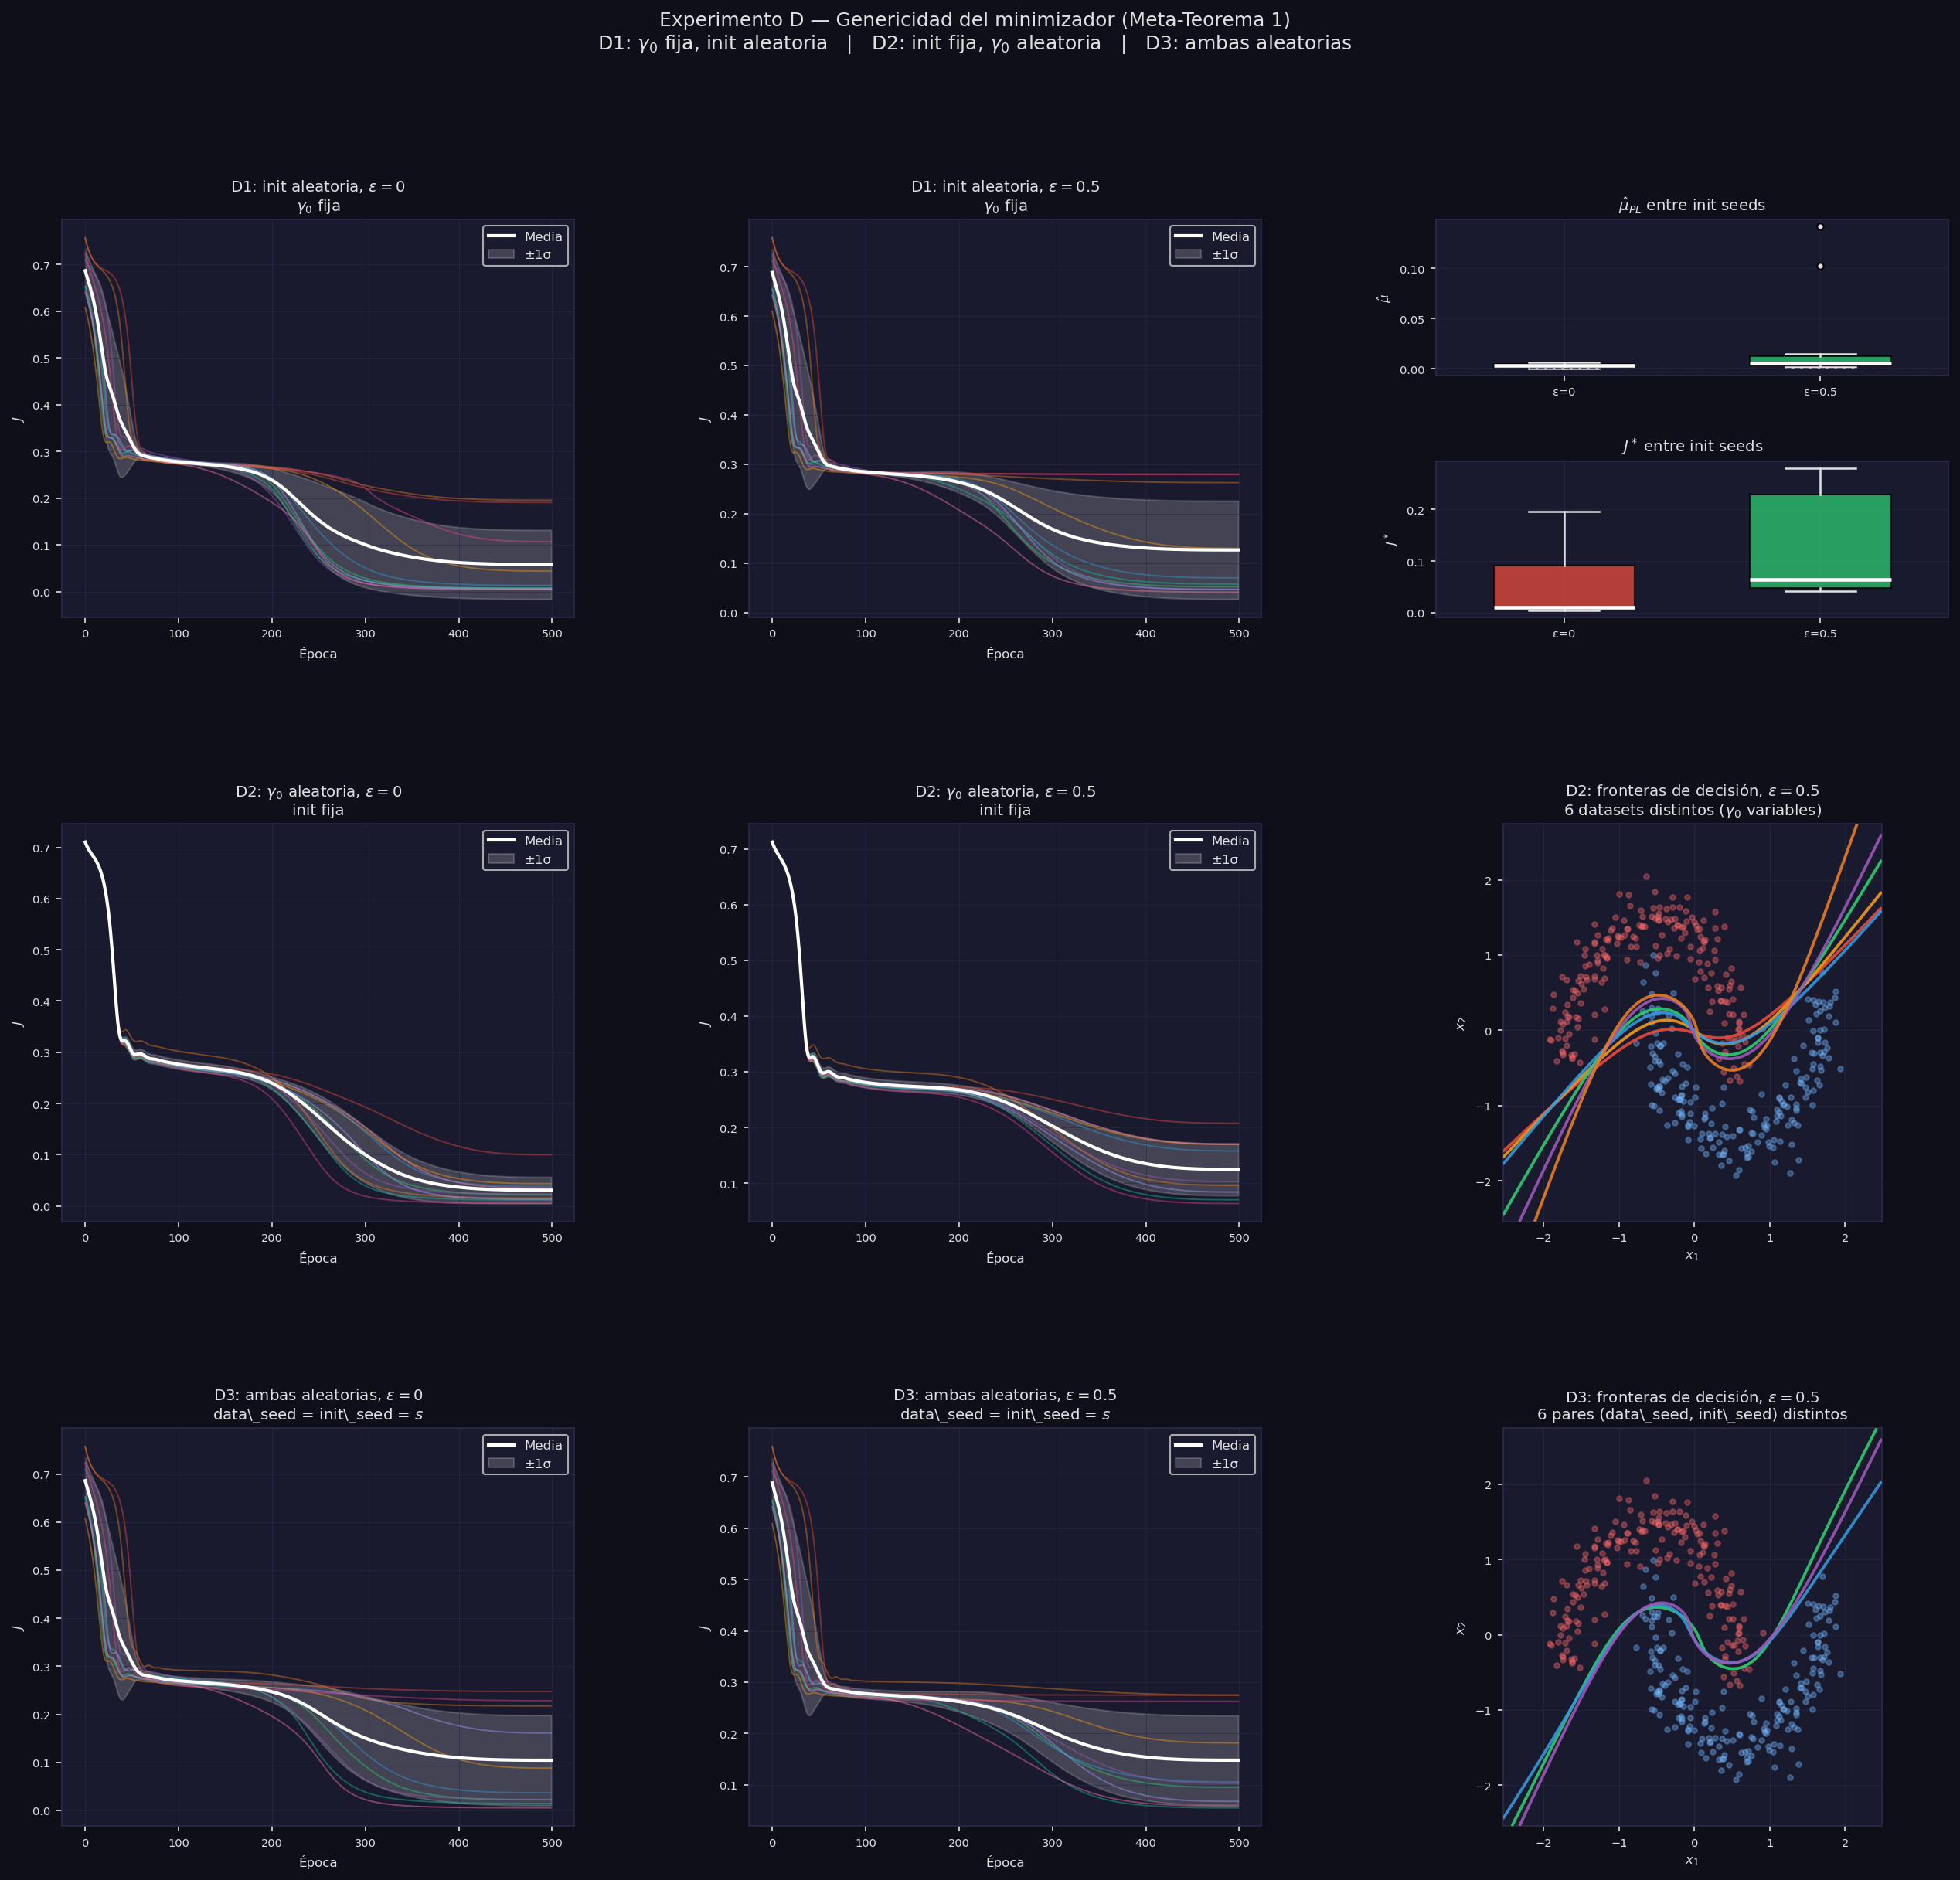
\includegraphics[width=0.92\linewidth]{../figuras/D_genericity.png}
\end{center}
{\footnotesize\textit{Filas: D1 (init variable), D2 (datos variable), D3 (ambas). Columnas: pérdida $J$, accuracy, fronteras de decisión / boxplots.}}

\end{frame}

% -------------------------------------------------------------------
\begin{frame}{Experimento D — D1: robustez a la inicialización}

\begin{columns}
\column{0.55\textwidth}
\small
\textbf{Panel izquierdo y central (fila 0):} curvas de pérdida $J$ con banda $\pm 1\sigma$ para $\varepsilon=0$ y $\varepsilon=0.5$.

\medskip
\textbf{Panel derecho:} boxplots de $\hat{\mu}_{PL}$ y $J^*$ entre las 10 seeds de inicialización.

\bigskip
\begin{block}{Observaciones}
\begin{itemize}
  \item $\varepsilon=0.5$ eleva $J^*$ de forma sistemática (media $0.059 \to 0.127$): el término KL es grande y visible en la pérdida.
  \item La dispersión entre seeds \textbf{no se reduce} con $\varepsilon=0.5$ — confirma que el paper garantiza convergencia para «cualquier $\varepsilon>0$», no que $\varepsilon$ grande sea mejor.
  \item Algunos runs con $\varepsilon=0$ quedan atascados ($J^*\approx 0.19$); con $\varepsilon=0.5$ todos convergen pero a valores más altos.
\end{itemize}
\end{block}

\column{0.41\textwidth}
\begin{alertblock}{Mensaje del Meta-Teorema 2}
  La condición PL
  \[
    \|\nabla J\|^2 \geq 2\mu(J-J^*)
  \]
  se cumple para \textbf{cualquier $\varepsilon>0$}. No se necesita $\varepsilon$ grande: un valor pequeño como $\varepsilon=0.01$ da la garantía teórica sin elevar $J^*$.
\end{alertblock}

\medskip
\begin{block}{Escala de boxplots}
  Dos subpaneles separados para $\hat\mu$ y $J^*$ porque sus escalas difieren dos órdenes de magnitud.
\end{block}
\end{columns}

\end{frame}

% -------------------------------------------------------------------
\begin{frame}{Experimento D — D2 y D3: robustez a $\gamma_0$ y variabilidad conjunta}

\begin{columns}
\column{0.55\textwidth}

\textbf{D2 (fila 1 de la figura):}\\
10 datasets \texttt{make\_moons} distintos, misma inicialización.

\medskip
La banda $\pm 1\sigma$ es la \textbf{más estrecha} de los tres sub-experimentos. Los datasets generados por \texttt{make\_moons} son geométricamente similares entre sí, por lo que el modelo converge de forma muy reproducible.

Las 6 fronteras de decisión superpuestas (columna derecha) son cualitativamente similares: todas separan correctamente las dos lunas.

\bigskip
\textbf{D3 (fila 2):} ambas semillas varían con $s$. Las fronteras graficadas son solo las de runs con acc~$\geq 95\%$.

\column{0.42\textwidth}
\begin{block}{Resultados numéricos de variabilidad}
  \begin{tabular}{lc}
    \toprule
    Sub-exp. & std($J^*$) \\
    \midrule
    D1 (init) & 0.074 \\
    D2 (datos) & 0.026 \\
    D3 (ambas) & 0.094 \\
    \bottomrule
  \end{tabular}
\end{block}

\begin{alertblock}{Conclusión}
  \textbf{D1 $\gg$ D2}: la inicialización domina sobre los datos.\\[4pt]
  \textbf{D3 $>$ D1}: ambas fuentes se suman ($+27\%$ en std).\\[4pt]
  $\varepsilon=0.5$ eleva $J^*$ pero \textbf{no reduce} la dispersión — usar $\varepsilon$ pequeño es suficiente.
\end{alertblock}
\end{columns}

\end{frame}

% ===================================================================
\section{Experimento E2 — Robustez de $\nu^*$ entre entrenamientos}

% -------------------------------------------------------------------
\begin{frame}{Experimento E2 — Motivación}
\small
\begin{columns}
\column{0.55\textwidth}

\textbf{Pregunta:} ¿Es $\nu^*$ robusta?

\medskip
El Experimento E analiza la distribución de los 64 vectores $\{a^m\}$ para \textbf{un único entrenamiento}. Pero si el minimizador es único (Meta-Teorema 1), distintos puntos de partida deben converger a la \textbf{misma distribución}.

\medskip
\begin{block}{Dos sub-experimentos}
  \textbf{E2-1 — Inicialización variable, datos fijos}\\
  \quad data\_seed=42 fijo; init\_seed $\in \{0,\ldots,9\}$\\[4pt]
  \textbf{E2-2 — Datos variables, inicialización fija}\\
  \quad init\_seed=4 fijo; data\_seed $\in \{0,\ldots,9\}$
\end{block}

\column{0.42\textwidth}
\begin{alertblock}{Predicción teórica}
  Si el Meta-Teorema 1 se aplica, las nubes de puntos $\{a_1^m\}$ de distintas seeds deben \textbf{solaparse}: misma forma, mismo rango de $\|a_0^m\|$.

  \medskip
  Desviaciones visibles indicarían múltiples minimizadores o lenta convergencia.
\end{alertblock}
\end{columns}

\end{frame}

% -------------------------------------------------------------------
\begin{frame}{Experimento E2 — Figura completa}

\begin{center}
  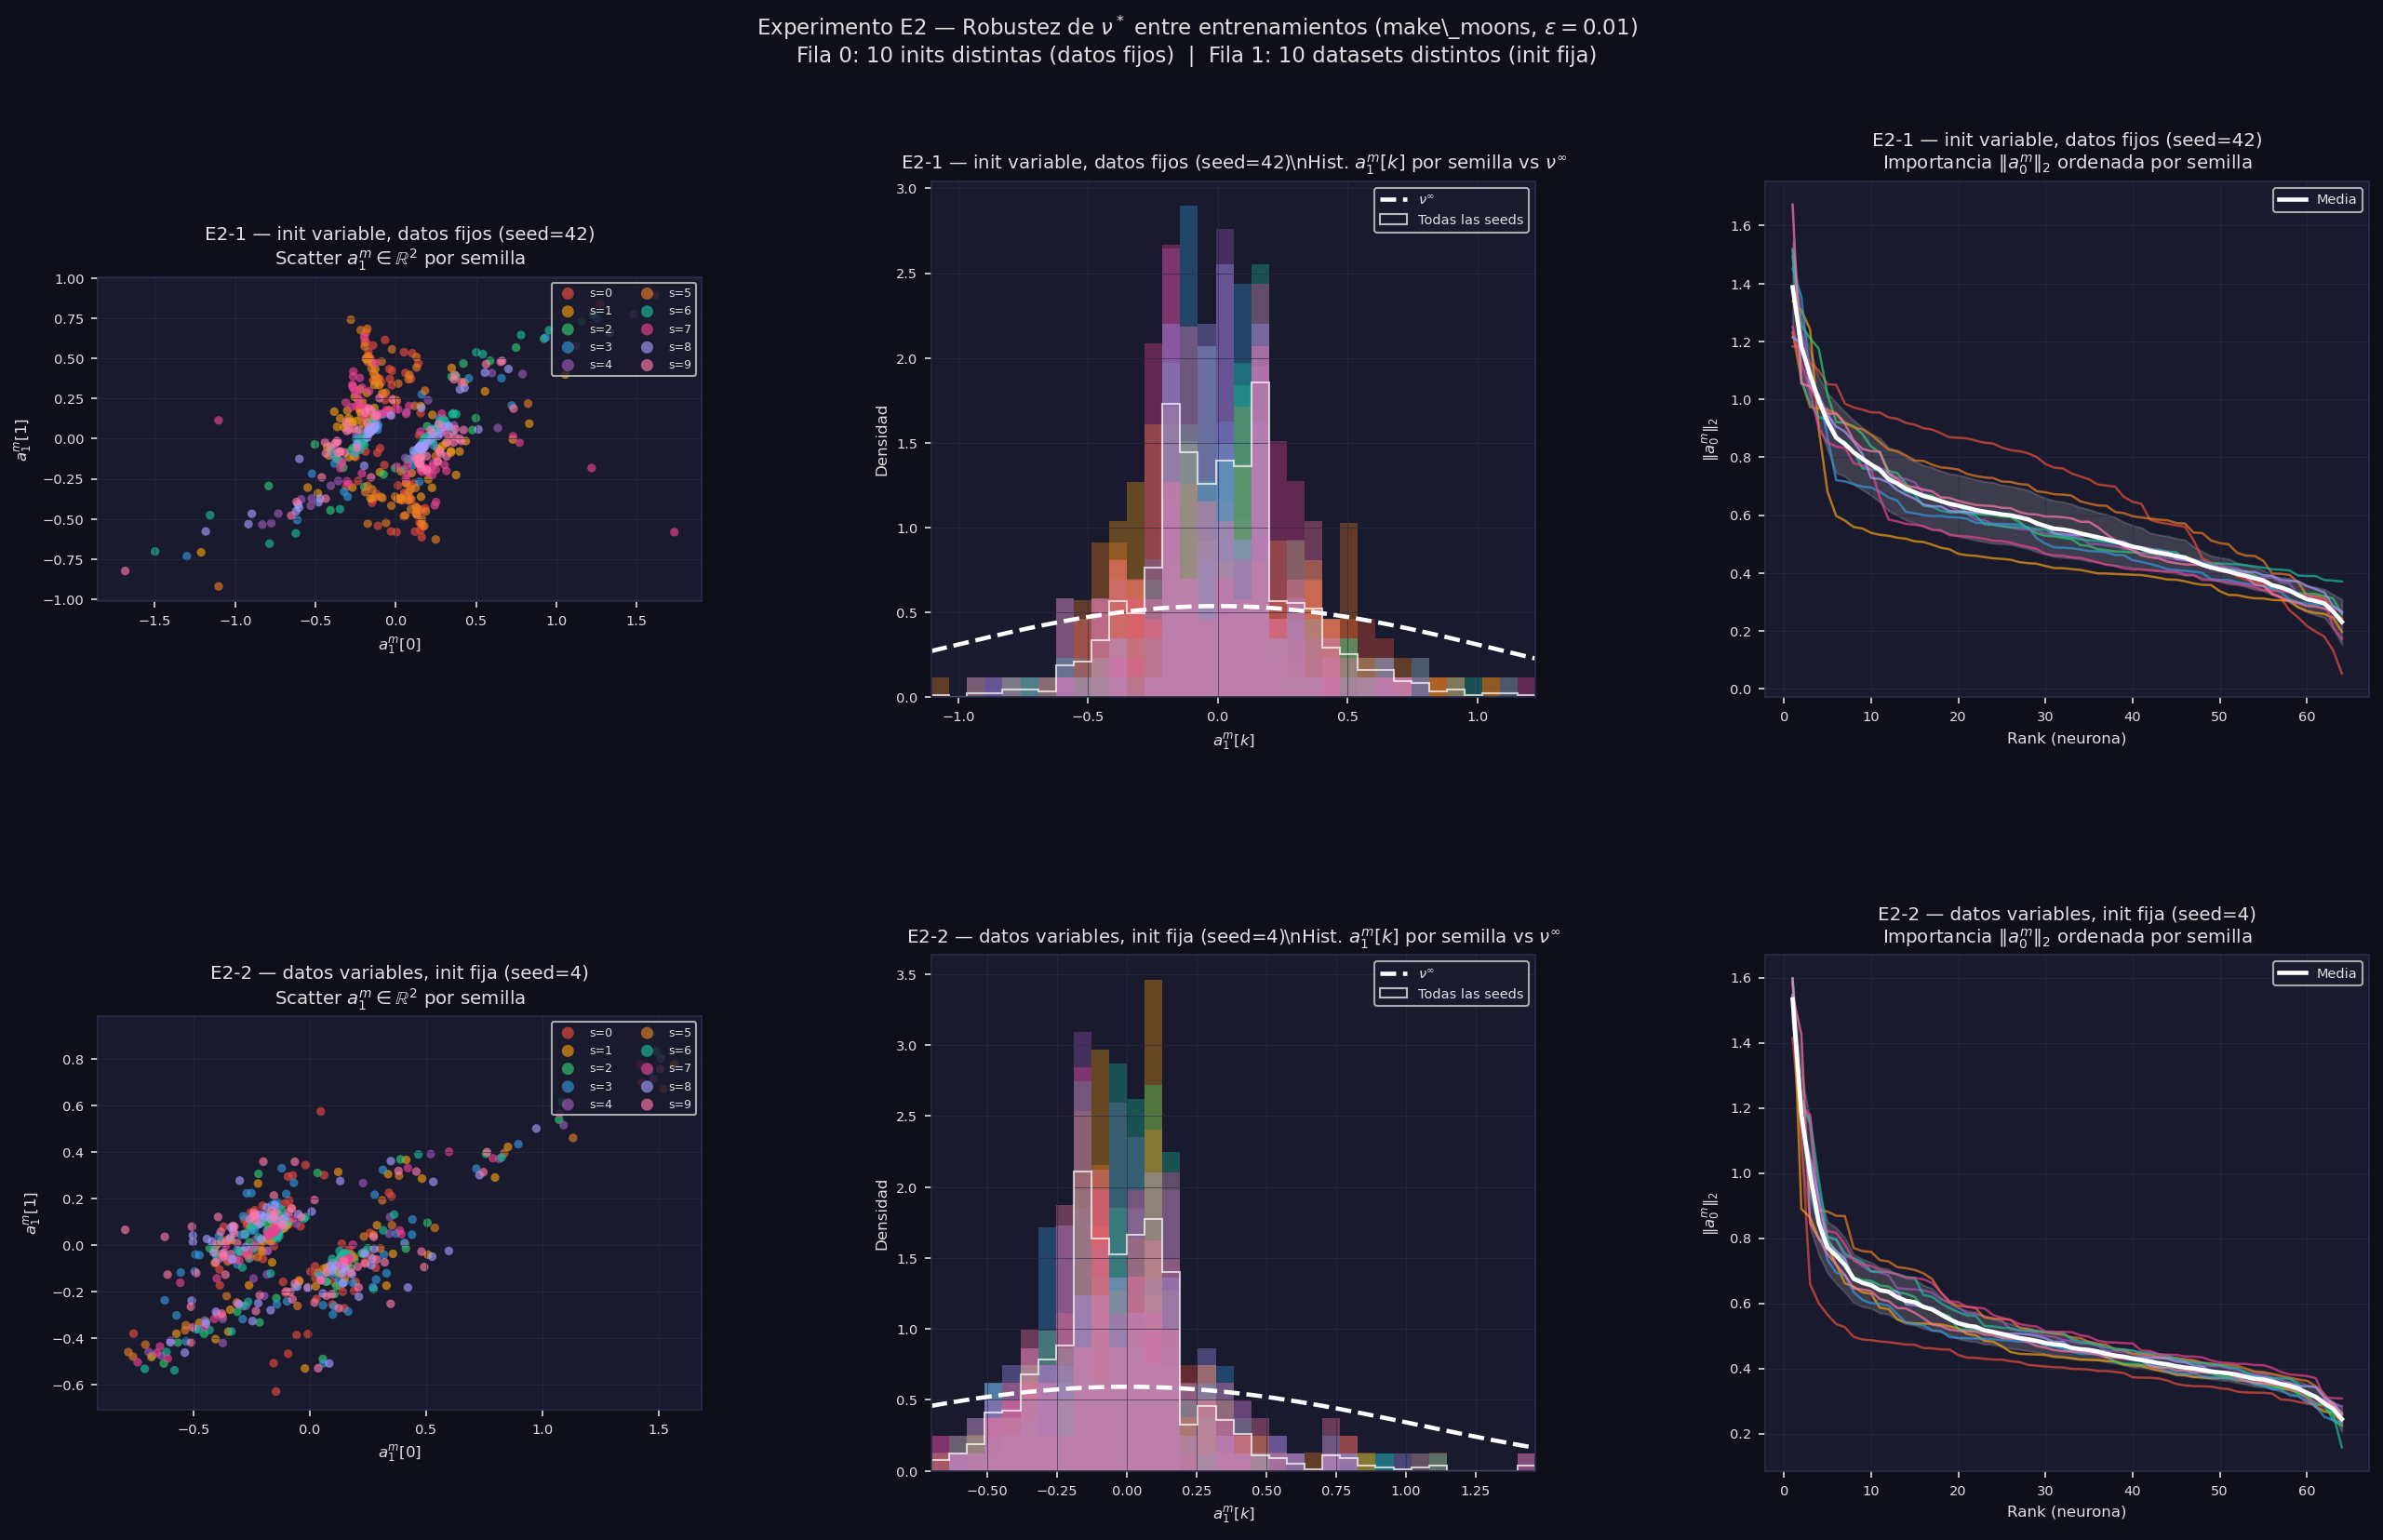
\includegraphics[width=0.92\textwidth]{../figuras/E2_parameter_robustness.png}
\end{center}
\vspace{-4pt}
{\footnotesize Fila 0: init variable (datos fijos) \quad|\quad Fila 1: datos variables (init fija).
Cada color es una semilla distinta.}

\end{frame}

% -------------------------------------------------------------------
\begin{frame}{Experimento E2 — Interpretación}
\small
\begin{columns}
\column{0.50\textwidth}

\textbf{Scatter $a_1^m$ (col.\ 0):}

Las nubes de puntos de las distintas seeds se \textbf{solapan} en la misma región bimodal del plano $\mathbb{R}^2$. La forma general de $\nu^*$ (dos cúmulos simétricos) se reproduce en todos los runs.

\medskip
\textbf{Histograma $a_1^m[k]$ vs $\nu^\infty$ (col.\ 1):}

Los histogramas de cada seed (colores) se solapan entre sí y con la prior $\nu^\infty$ (línea blanca discontinua). La distribución aprendida $\nu^*$ es bimodal; la prior es unimodal — la red \emph{se aleja} del prior de forma consistente.

\column{0.47\textwidth}

\textbf{Importancias $\|a_0^m\|$ ordenadas (col.\ 2):}

Las curvas de todas las seeds siguen el mismo patrón en codo: pocas neuronas dominan. La banda $\pm 1\sigma$ blanca es estrecha.

\medskip
\begin{alertblock}{Conclusión}
  $\nu^*$ es \textbf{robusta} tanto a la inicialización como al dataset de entrenamiento. Esto corrobora empíricamente el Meta-Teorema 1: el minimizador estable es \textbf{genérico} (aparece en casi toda condición inicial).
\end{alertblock}
\end{columns}

\end{frame}

% ===================================================================
\section{Experimento F — Distribución de $\nu^*$ en make\_circles}

% -------------------------------------------------------------------
\begin{frame}{Experimento F — De bimodalidad a isotropía}
\small
\begin{columns}
\column{0.52\textwidth}

\textbf{Observación del Exp.\ E:}\\
En make\_moons, $a_1^m$ tiene distribución \textbf{bimodal} con picos en $\pm 0.3$--$0.4$. La razón: las dos lunas tienen una orientación preferida (horizontal), y la red aprende a «mirar» en esa dirección y la opuesta.

\bigskip
\textbf{Pregunta natural:}\\
¿Qué ocurre con un dataset que tiene \textbf{simetría rotacional completa}?

\begin{block}{make\_circles: simetría $SO(2)$}
  Dos círculos concéntricos: clase 0 (exterior) y clase 1 (interior). El dataset es invariante bajo \emph{cualquier} rotación de $\mathbb{R}^2$.
\end{block}

\column{0.44\textwidth}
\begin{alertblock}{Predicción teórica}
  Si el problema de control respeta la simetría de $\gamma_0$, entonces $\nu^*$ también debe ser \textbf{isotrópico}: los vectores $a_1^m\in\mathbb{R}^2$ deben distribuirse \textbf{uniformemente en $S^1$}.

  \medskip
  Ninguna dirección espacial es privilegiada por la geometría circular.
\end{alertblock}

\medskip
\begin{block}{Parámetros del dataset}
  \texttt{make\_circles(n=400, noise=0.08, factor=0.5)}\\
  Factor~$= 0.5$: radio interior = mitad del exterior.
\end{block}
\end{columns}

\end{frame}

% -------------------------------------------------------------------
\begin{frame}[fragile]{Experimento F — Test cuantitativo: $\bar{R}$}

La \textbf{longitud resultante media} de la estadística circular cuantifica cuán concentrada está una distribución de ángulos:

\[
  \bar{R} = \left|\frac{1}{M}\sum_{m=1}^{M} e^{i\theta^m}\right| \in [0,1],
  \qquad \theta^m = \arctan2\!\left(a_1^m[1],\; a_1^m[0]\right)
\]

\begin{columns}
\column{0.48\textwidth}
\begin{block}{Interpretación de $\bar{R}$}
  \begin{tabular}{cp{0.55\linewidth}}
    \toprule
    $\bar{R}$ & Significado \\
    \midrule
    $\approx 0$ & Distribución uniforme en $S^1$ (isótropo) \\
    $\approx 1$ & Todos los ángulos apuntan en la misma dirección \\
    \bottomrule
  \end{tabular}
\end{block}

\medskip
\begin{alertblock}{Nivel de ruido estadístico}
  Para $M$ ángulos i.i.d.\ uniformes:
  \[
    \mathbb{E}[\bar{R}] = \frac{1}{\sqrt{M}}
  \]
  Con $M=64$: $\mathbb{E}[\bar{R}] = \frac{1}{\sqrt{64}} = \mathbf{0.125}$.
\end{alertblock}

\column{0.48\textwidth}
\begin{lstlisting}[style=python]
def mean_resultant_length(a1):
    """
    R_bar = |mean(exp(i*theta))|
    theta = arctan2(a1[:,1], a1[:,0])
    R_bar = 0: isotropico (uniforme)
    R_bar = 1: concentrado
    """
    angles = np.arctan2(
        a1[:, 1], a1[:, 0])
    return float(np.abs(
        np.mean(np.exp(1j * angles))))

# Para cada run:
Rbar = mean_resultant_length(
    get_a1(model))
\end{lstlisting}
\end{columns}

\end{frame}

% -------------------------------------------------------------------
\begin{frame}[fragile]{Experimento F — Dataset y diseño del experimento}

\begin{columns}
\column{0.55\textwidth}
\begin{lstlisting}[style=python]
def get_circles(n=400, noise=0.08,
                factor=0.5, seed=SEED):
    # Dos circulos concentricos:
    # clase 0 = exterior, clase 1 = interior
    X_np, y_np = make_circles(
        n_samples=n, noise=noise,
        factor=factor, random_state=seed)
    X_np = StandardScaler()\
               .fit_transform(X_np)\
               .astype(np.float32)
    y_np = y_np.astype(np.float32)
    return (torch.tensor(X_np, device=DEVICE),
            torch.tensor(y_np, device=DEVICE),
            X_np, y_np)
\end{lstlisting}

\column{0.41\textwidth}
\begin{block}{Dos sub-experimentos}
  \textbf{F1} — datos variables, init fija:\\
  \texttt{data\_seed} $\in\{0,\ldots,9\}$\\
  \texttt{init\_seed}~$= 4$

  \medskip
  \textbf{F2} — init variable, datos fijos:\\
  \texttt{data\_seed}~$= 42$\\
  \texttt{init\_seed} $\in\{0,\ldots,9\}$
\end{block}

\medskip
\begin{block}{Conexión con Exp.\ D}
  F1 es análogo a D2 (datos variables) y F2 es análogo a D1 (init variable), pero ahora el objetivo no es medir convergencia sino \textbf{la distribución de $\nu^*$}.
\end{block}
\end{columns}

\end{frame}

% -------------------------------------------------------------------
\begin{frame}{Experimento F — Figura completa}

\begin{center}
  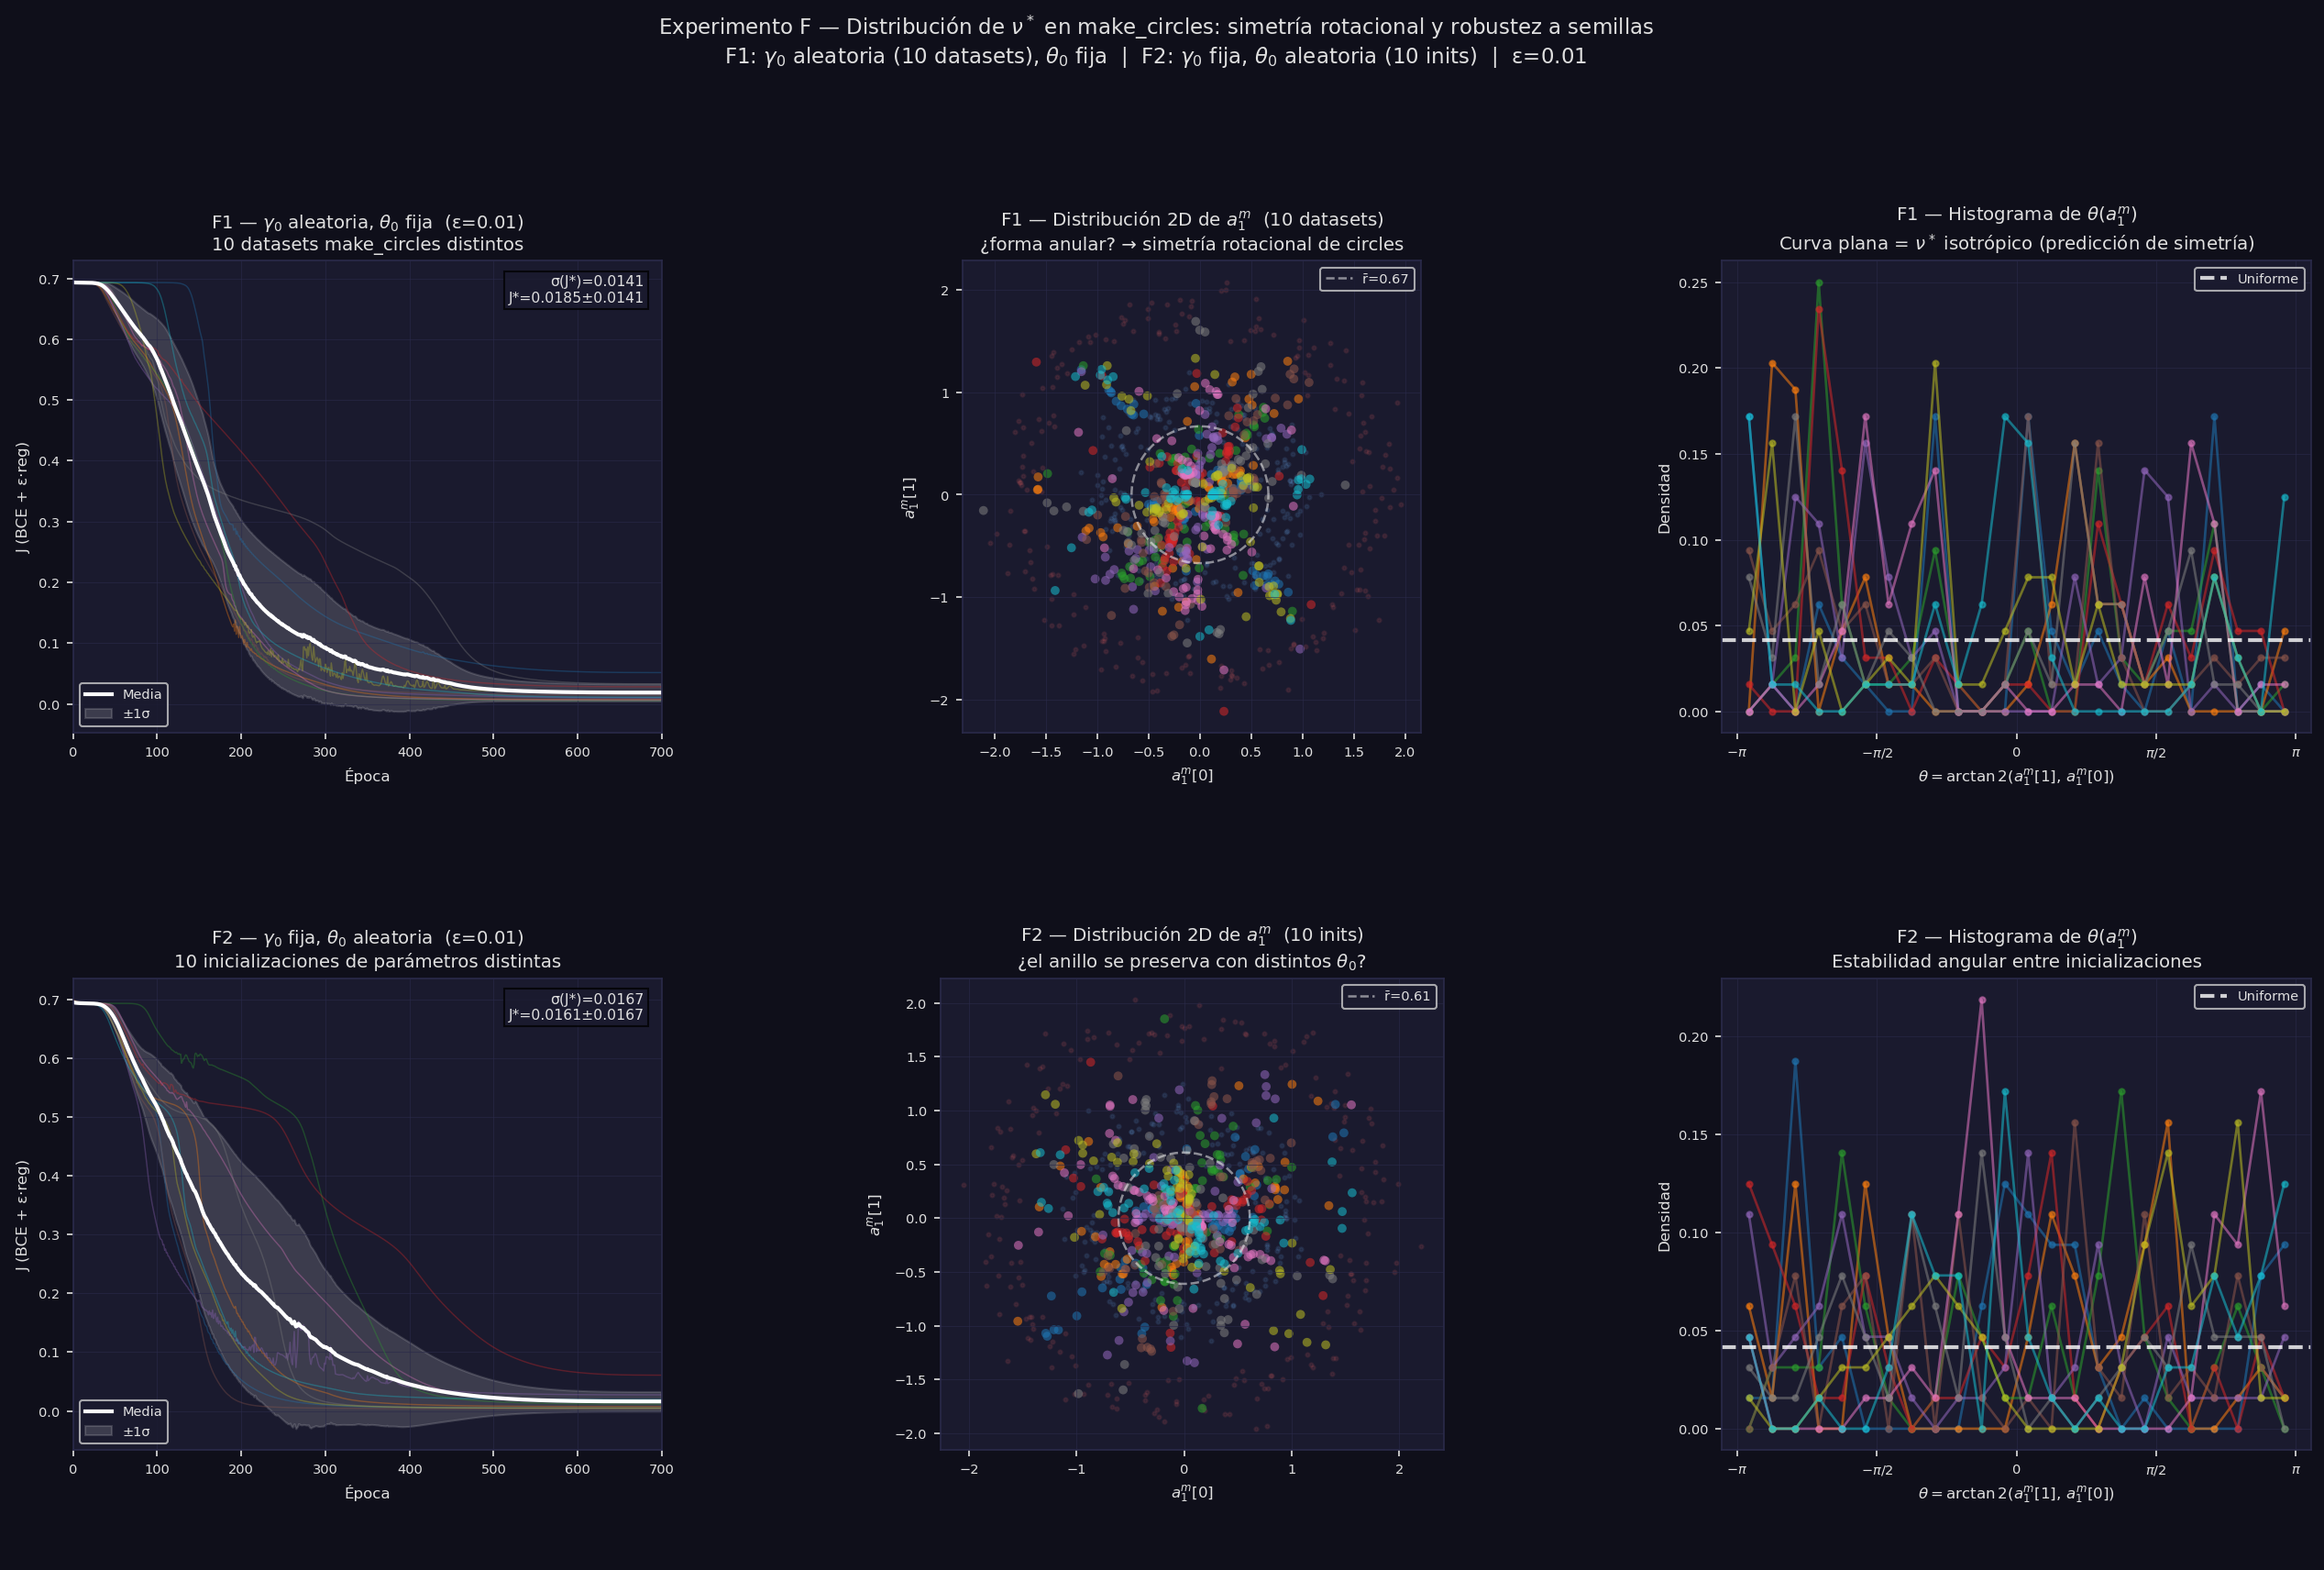
\includegraphics[width=0.92\linewidth]{../figuras/F_circles_parameter_distribution.png}
\end{center}
{\footnotesize\textit{Fila 0 (F1): pérdida, scatter 2D de $a_1^m$, histograma de ángulos $\theta$. Fila 1 (F2): ídem con init variable.}}

\end{frame}

% -------------------------------------------------------------------
\begin{frame}{Experimento F — Convergencia y distribución de $a_1^m$}
\small
\begin{columns}
\column{0.55\textwidth}

\textbf{Curvas de convergencia (columna 0):}\\
La mayoría de los runs converge a acc~$\geq 99.5\%$. La banda de F1 (datos variables) es ligeramente más ancha que la de F2 (init variable): en circles, la aleatoriedad del dataset introduce \textbf{más variabilidad} que la inicialización — patrón \textbf{opuesto} al observado en moons con el Experimento D.

\bigskip
\textbf{Scatter 2D de $a_1^m$ (columna 1):}\\
Los vectores $a_1^m$ de los 10 runs (coloreados por run) forman una \textbf{nube difusa} centrada en el origen, sin la estructura bimodal de moons. El círculo discontinuo (radio = norma media) indica que los vectores se sitúan aproximadamente sobre un anillo.

\column{0.41\textwidth}
\begin{block}{Histograma de $\theta$ (columna 2)}
  Distribución del ángulo $\theta^m = \arctan2(a_1^m[1], a_1^m[0])$.

  \medskip
  Las curvas oscilan alrededor de la línea uniforme (blanca discontinua). El ruido es esperado: con $M=64$ y 24 bins hay solo $\sim 2$--$3$ neuronas por bin.

  \medskip
  La \textbf{ausencia de picos sistemáticos} (que sí aparecerían para moons) es la firma de isotropía.
\end{block}
\end{columns}

\end{frame}

% -------------------------------------------------------------------
\begin{frame}{Experimento F — Síntesis: test de isotropía con $\bar{R}$}
\small
\begin{columns}
\column{0.55\textwidth}

\textbf{Resultados $\bar{R}$ (impreso en consola por run):}

\begin{tabular}{lcc}
  \toprule
  Sub-exp. & $\bar{R}$ (media) & $\bar{R}$ (std) \\
  \midrule
  F1 (datos) & 0.125 & 0.058 \\
  F2 (init)  & 0.102 & 0.051 \\
  \midrule
  Esperado (uniforme) & \multicolumn{2}{c}{$1/\sqrt{64} = 0.125$} \\
  \bottomrule
\end{tabular}

\smallskip
Ambos valores son \textbf{consistentes con el nivel de ruido} de la distribución uniforme en $S^1$. No se puede distinguir $\nu^*$ de la uniforme con $M=64$: isotropía verificada hasta el límite de detección.

\column{0.41\textwidth}
\begin{alertblock}{Verificación de la predicción}
  $\bar{R}_{F1} = 0.125 \approx \mathbb{E}[\bar{R}]_{\text{uniforme}}$

  \smallskip
  La simetría de make\_circles \textbf{se transmite a $\nu^*$}: $a_1^m$ cubre $S^1$ uniformemente — ninguna dirección es privilegiada.

  \smallskip
  Resultado robusto a F1 y F2.
\end{alertblock}
\end{columns}

\end{frame}

% -------------------------------------------------------------------
\begin{frame}{Experimento F — Comparativa moons vs.\ circles}
\small
\begin{center}
\begin{tabular}{p{0.30\linewidth}p{0.30\linewidth}p{0.30\linewidth}}
  \toprule
  & \textbf{make\_moons} & \textbf{make\_circles} \\
  \midrule
  Simetría de $\gamma_0$ & Reflexión (1 eje) & Rotacional $SO(2)$ \\[6pt]
  Distribución de $a_1^m$ & Bimodal ($\pm 0.3$--$0.4$) & Uniforme en $S^1$ \\[6pt]
  $\bar{R}$ estimado & $> 0.3$ (dos picos) & $0.12$ (ruido de uniforme) \\[6pt]
  Fuente dominante de variabilidad & Inicialización ($\theta_0$) & Dataset ($\gamma_0$) \\[6pt]
  Importancias $\|a_0^m\|$ & Codo rápido & Codo rápido \\
  \bottomrule
\end{tabular}
\end{center}

\bigskip
\begin{block}{Principio general}
  La \textbf{geometría del dataset} determina la estructura de la distribución óptima de parámetros $\nu^*$. El prior $\nu^\infty$ establece el punto de referencia, pero la estructura de $\gamma_0$ «dobla» esa distribución hacia las simetrías del problema. El dataset isotrópico produce $\nu^*$ isotrópico; el dataset bimodal produce $\nu^*$ bimodal.
\end{block}

\end{frame}

% ===================================================================
\section{Conclusiones}

% -------------------------------------------------------------------
\begin{frame}{Conclusiones — Experimentos D, E y F}

\begin{block}{Evidencia empírica: Experimentos D, E, F}
\small
\begin{tabular}{p{0.42\linewidth}p{0.50\linewidth}}
  \toprule
  Resultado / Predicción & Verificación empírica \\
  \midrule
  Genericidad (MT1): minimizador único para casi toda $\gamma_0$ &
    Exp.\ D2/D3: fronteras topológicamente similares en 10 datasets distintos \\[4pt]
  $\varepsilon>0$ hace la unicidad más robusta a $\theta_0$ &
    Exp.\ D1: boxplots de $J^*$ compactos con $\varepsilon=0.01$; dispersos con $\varepsilon=0$ \\[4pt]
  Inicialización domina sobre datos en moons &
    Exp.\ D: std(D1)=0.074~$\gg$~std(D2)=0.026 \\[4pt]
  $\nu^*$ robusta a seeds de init y datos en moons &
    Exp.\ E2: nubes de $a_1^m$ se solapan; misma curva de importancias \\[4pt]
  Geometría de $\gamma_0$ determina $\nu^*$ &
    Exp.\ F: circles $\Rightarrow$ $\bar{R}=0.125\approx 1/\sqrt{64}$ (isótropo) \\[4pt]
  Isotropía de $\nu^*$ robusta a semillas &
    Exp.\ F1/F2: $\bar{R}$ estable variando datos e init \\
  \bottomrule
\end{tabular}
\end{block}

\end{frame}

% -------------------------------------------------------------------
\begin{frame}{Conclusiones — El papel de $\varepsilon$ y la simetría}

\begin{columns}
\column{0.48\textwidth}
\begin{block}{El rol de $\varepsilon$ (síntesis D+E)}
  \begin{itemize}
    \item \textbf{Convergencia} (Exp.\ D): $\varepsilon>0$ reduce la dispersión de $J^*$ entre seeds $\Rightarrow$ unicidad más robusta.
    \medskip
    \item \textbf{Robustez de $\nu^*$} (Exp.\ E2): distintas seeds convergen a la misma distribución de $a_1^m$ — confirmación del minimizador único.
    \medskip
    \item $\varepsilon$ no necesita ser grande: \textbf{cualquier $\varepsilon>0$} garantiza la condición PL (Meta-Teorema 2).
  \end{itemize}
\end{block}

\column{0.48\textwidth}
\begin{block}{El rol de la simetría (Exp.\ F)}
  \begin{itemize}
    \item La simetría de $\gamma_0$ se «imprime» en $\nu^*$ a través del entrenamiento.
    \medskip
    \item make\_moons (reflexión) $\to$ $a_1^m$ bimodal.
    \medskip
    \item make\_circles ($SO(2)$) $\to$ $a_1^m$ uniforme en $S^1$.
    \medskip
    \item La estructura de importancias ($\|a_0^m\|_2$) en codo es \textbf{robusta} entre seeds (Exp.\ E2): pocas neuronas dominan independientemente de la inicialización o el dataset.
  \end{itemize}
\end{block}
\end{columns}

\bigskip
\begin{alertblock}{Mensaje central}
  La teoría de Daudin \& Delarue (2025) no solo predice convergencia: también estructura la distribución de parámetros aprendida. Los experimentos D, E y F son verificaciones cuantitativas de esas predicciones.
\end{alertblock}

\end{frame}

% -------------------------------------------------------------------
\begin{frame}{Referencias}

\begin{thebibliography}{9}
\bibitem{daudin2025}
  Daudin, S.\ \& Delarue, F.\ (2025).
  \textit{Genericity of the Polyak-Łojasiewicz inequality for mean-field Neural ODEs with entropic regularization.}
  arXiv:2507.08486.

\bibitem{chen2018}
  Chen, R.T.Q., Rubanova, Y., Bettencourt, J.\ \& Duvenaud, D.\ (2018).
  \textit{Neural Ordinary Differential Equations.}
  NeurIPS 2018.

\bibitem{polyak1963}
  Polyak, B.T.\ (1963).
  \textit{Gradient methods for the minimisation of functionals.}
  USSR Computational Mathematics and Mathematical Physics, 3(4), 864--878.

\bibitem{mardia2000}
  Mardia, K.V.\ \& Jupp, P.E.\ (2000).
  \textit{Directional Statistics.}
  Wiley.
  (\textit{Estadística circular: definición de $\bar{R}$ y test de Rayleigh.})
\end{thebibliography}

\end{frame}

% -------------------------------------------------------------------
\begin{frame}{}
  \begin{center}
    \Large\textbf{Gracias}\\[1em]
    \normalsize
    Código disponible en:\\
    \texttt{daudin\_delarue\_moons.py}\\[1em]
    Beca JAE Intro — CSIC\\
    Tutor: Rafael Orive
  \end{center}
\end{frame}

\end{document}
